\documentclass[conference]{IEEEtran}
\IEEEoverridecommandlockouts

\usepackage[spanish,es-nodecimaldot,es-noshorthands]{babel}
\usepackage[utf8]{inputenc}
\usepackage[T1]{fontenc}
\usepackage{amsmath,amssymb}
\usepackage{graphicx}
\usepackage{xcolor}
\usepackage{float}
\usepackage{array}
\usepackage[hidelinks]{hyperref}

\definecolor{gris}{rgb}{0.45,0.45,0.45}
% Espacio reservado para la captura con el hardware real.
\newcommand{\imgph}[2]{%
	\fbox{\begin{minipage}[c][#2][c]{0.92\columnwidth}
			\centering\textcolor{gris}{\footnotesize [Espacio para imagen: #1]}
	\end{minipage}}%
}
\newcommand{\hw}{\textcolor{gris}{Pendiente}}

\begin{document}

\title{Avance 2: Módulo de Adquisición del Mando \\
	\large Terminal de Juegos Retro Distribuida con Mando Embebido}

\author{
	\IEEEauthorblockN{Belmont Muñoz Samuel}
	\IEEEauthorblockA{No. Cuenta: 317318289}
	\and
	\IEEEauthorblockN{Domínguez Palacios Jesús Alejandro}
	\IEEEauthorblockA{No. Cuenta: 421066205}
	\and
	\IEEEauthorblockN{Dorantes Mejía Emmanuel}
	\IEEEauthorblockA{No. Cuenta: 313004766}
	\and
	\IEEEauthorblockN{García Olvera Emiliano}
	\IEEEauthorblockA{No. Cuenta: 314256009}
	\and
	\IEEEauthorblockN{Hernández Alonso Antonio Adonahí}
	\IEEEauthorblockA{No. Cuenta: 316339825}
	\and
	\IEEEauthorblockN{Jiménez Reyes Alan Yael}
	\IEEEauthorblockA{No. Cuenta: 320026726}
}

\maketitle

\begin{center}
	\vspace{-0.3cm}
	{\small \textbf{Fundamentos de Sistemas Embebidos, Grupo 6} \quad
	\textbf{Fecha:} 04/11/2026}
\end{center}

\begin{abstract}
Este avance demuestra el módulo de adquisición del mando: una Raspberry Pi Pico lee los botones por registros 74HC165 cada $5\text{ ms}$, sin intervención manual. El módulo cumple el requisito funcional 1 del Avance 1. Aquí documentamos el cableado, la configuración, las pruebas y las decisiones que el código aplica.
\end{abstract}

\begin{IEEEkeywords}
Raspberry Pi Pico, PIO, 74HC165, bare-metal, antirrebote.
\end{IEEEkeywords}

\section{Módulo demostrado}

\textbf{Requisito que cumple:} leer todos los botones con un periodo de $5\text{ ms} \pm 0.5\text{ ms}$, o sea a $200\text{ Hz}$ estables.

La versión anterior ya leía bien el registro, pero iba a ritmo de depuración, con un bit visible cada tanto. Esta versión hace lo mismo en menos de $20\text{ }\mu\text{s}$ y lo repite por temporizador.

El módulo arranca solo al recibir energía. Core 1 captura y filtra los botones por interrupciones. Core 0 manda cada segundo un resumen por USB serial, mueve el LED y alimenta al watchdog. Si dejan de llegar muestras durante $2\text{ s}$, la Pico se reinicia sola. El script \texttt{verificar\_modulo.sh} lee ese resumen y responde PASA o FALLA, sin que nadie interprete los números.

\begin{figure}[H]
	\centering
	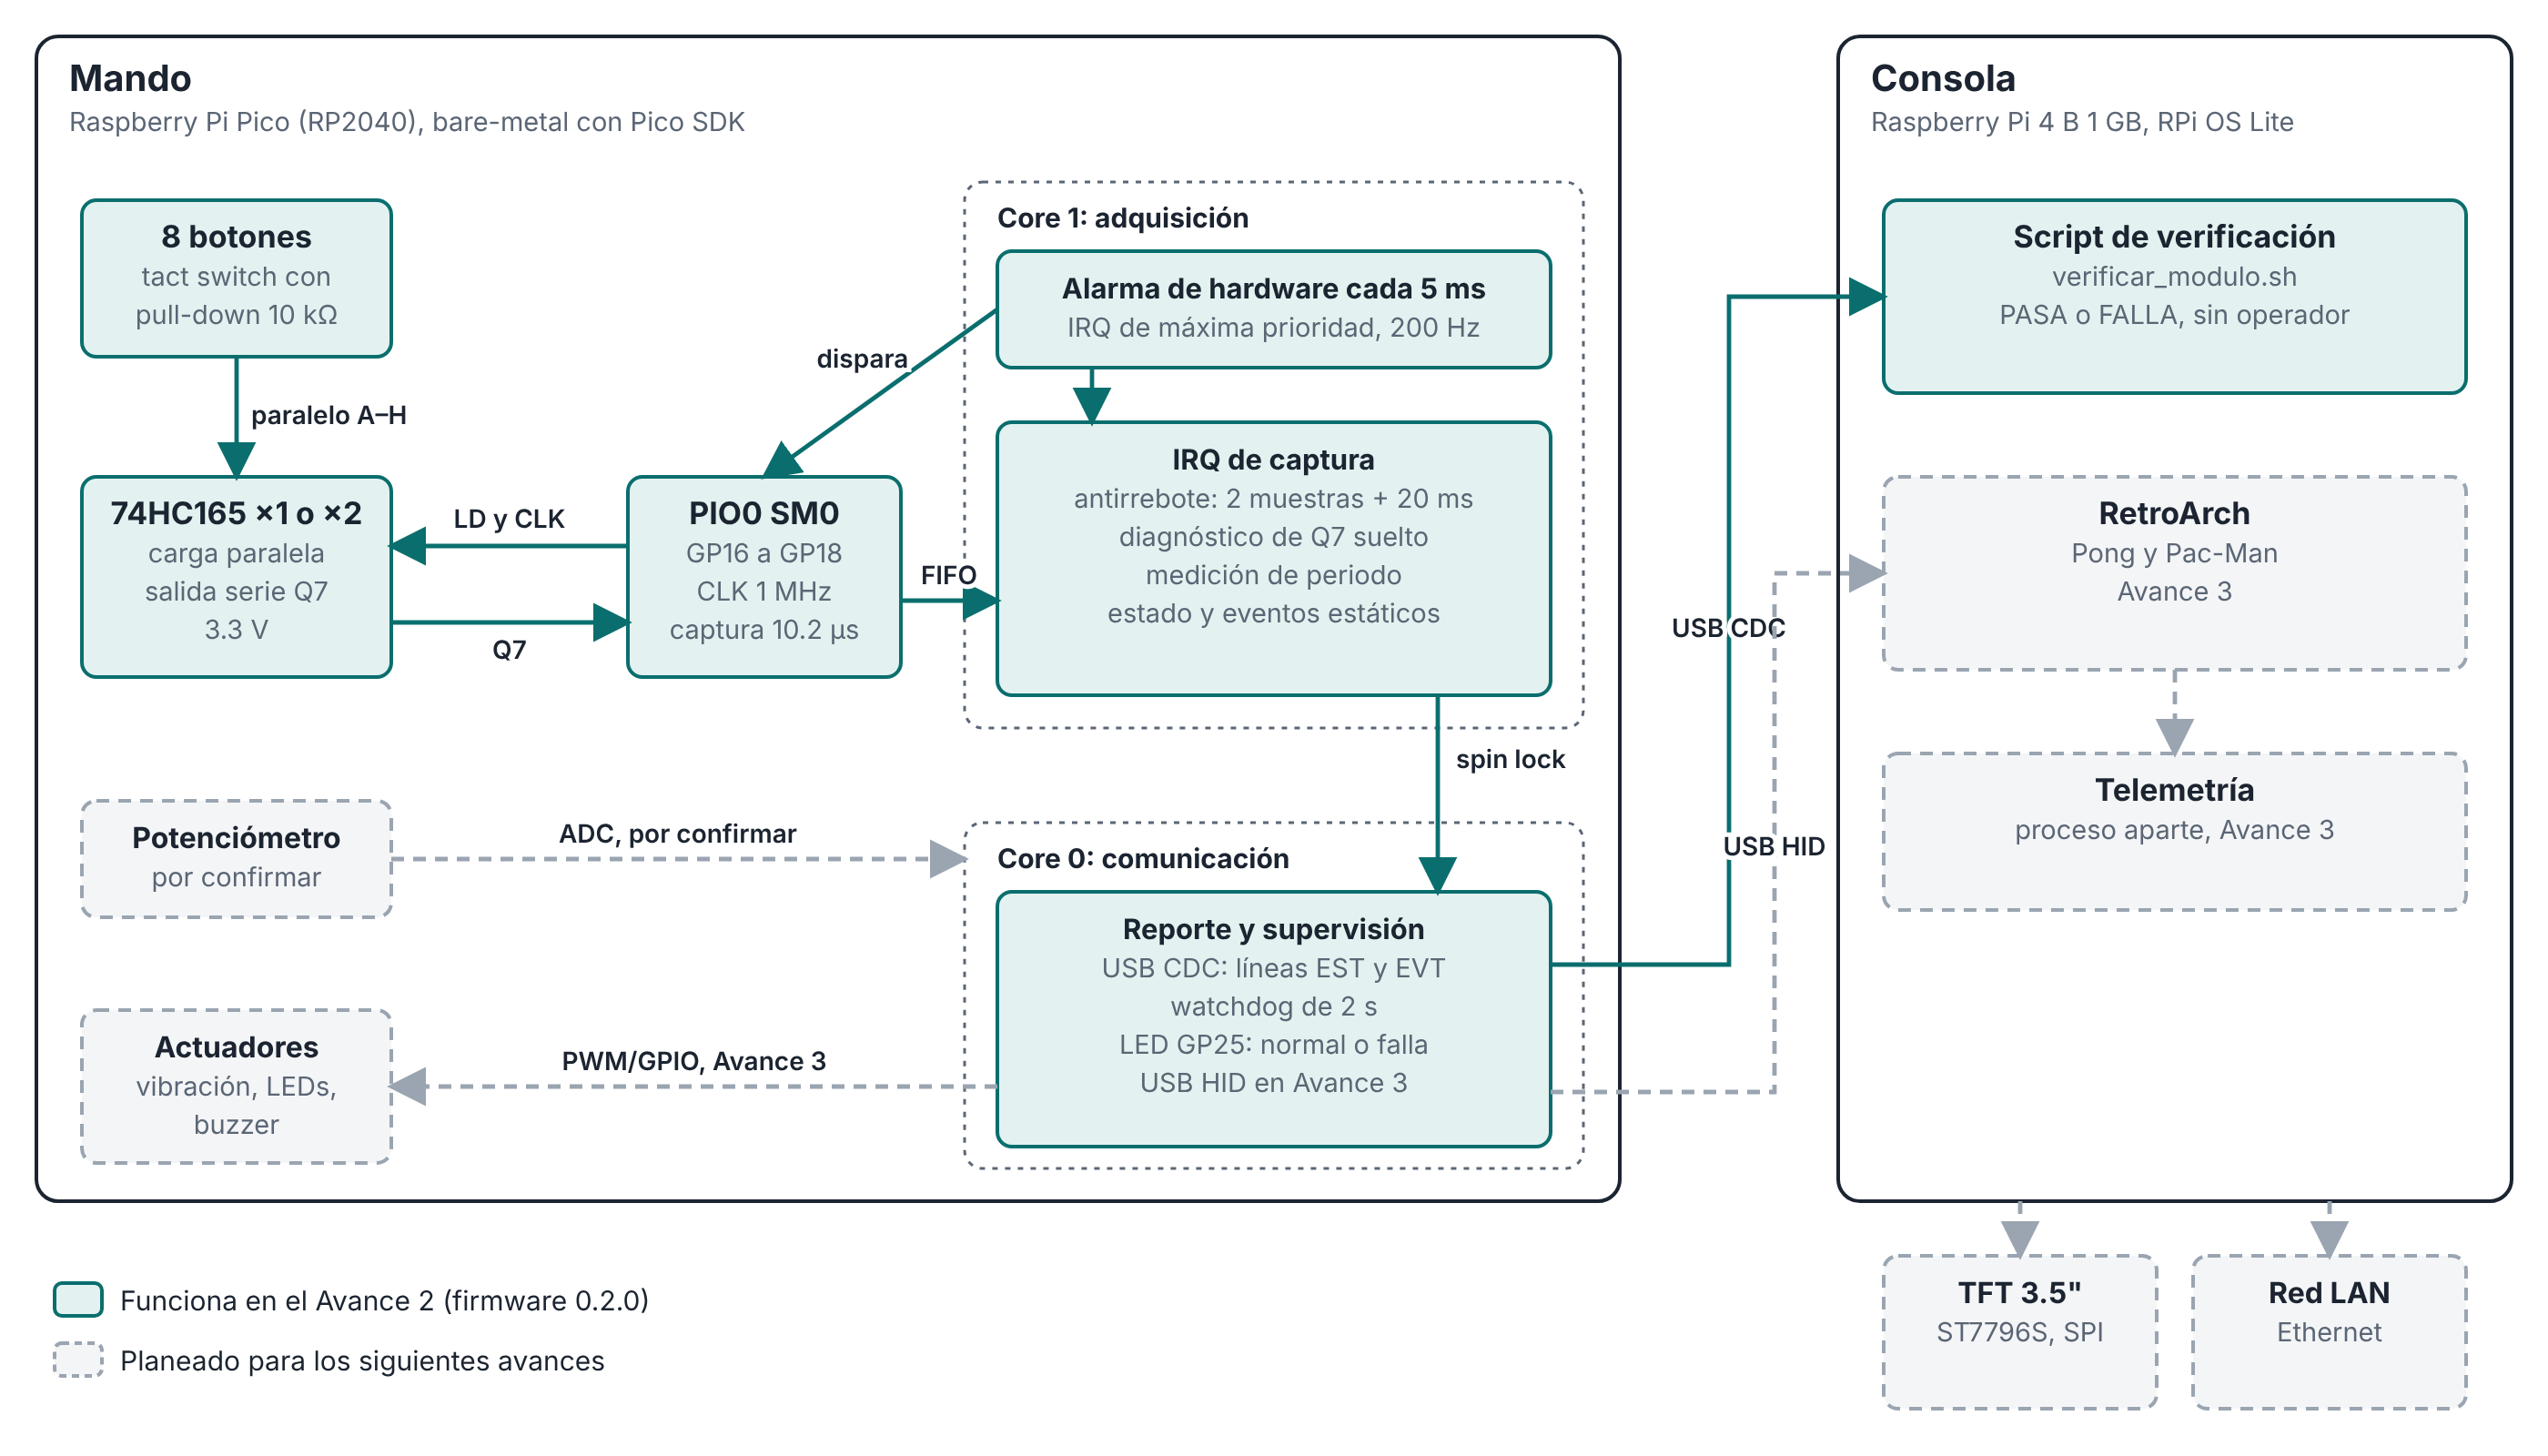
\includegraphics[width=\columnwidth]{img/diagrama_bloques.png}
	\caption{Diagrama de bloques actualizado.}
	\label{fig:bloques}
\end{figure}

\begin{table*}[!t]
	\centering
	\caption{Casos de prueba: esperado y obtenido}
	\label{tab:pruebas}
	\small
	\begin{tabular}{|c|p{4.3cm}|p{4cm}|p{5.2cm}|p{1.6cm}|}
		\hline
		\textbf{Caso} & \textbf{Prueba} & \textbf{Esperado} & \textbf{Obtenido en emulador o PC} & \textbf{Hardware} \\
		\hline
		P1 & Reposo, midiendo LD externamente & $200\text{ Hz}$, periodo de $4{,}500$ a $5{,}500\text{ }\mu\text{s}$ & $5{,}000.0\text{ }\mu\text{s}$ promedio, de $4{,}998.2$ a $5{,}001.8$; $n=2{,}419$; 0 perdidas & \hw \\
		\hline
		P2 & Protocolo por captura & 8 flancos de CLK a $1\text{ MHz}$ (16 con dos chips) & 8 de 8 en $2{,}517$ capturas; 16 de 16 en $2{,}837$; CLK de $1.000\text{ }\mu\text{s}$ & \hw \\
		\hline
		P3 & Un botón a la vez, en todos los bits & Cada bit en su posición & 8 de 8 y 16 de 16 correctos & \hw \\
		\hline
		P4 & 40 pulsaciones en fases distintas & Retardo $\le 10\text{ ms}$ & De $5.03$ a $9.96\text{ ms}$; promedio $7.38\text{ ms}$ & \hw \\
		\hline
		P5 & Pruebas de lógica con sanitizadores & Sin fallas & $2{,}040$ verificaciones, 0 fallas (PC) & No aplica \\
		\hline
		F1 & \textbf{Falla:} Q7 desconectado $2\text{ s}$ & \texttt{abierta=1}, sin botones fantasma, se recupera solo & \texttt{abierta=1}, 0 eventos, \texttt{abierta=0} al reconectar & \hw \\
		\hline
		F2 & \textbf{Falla:} rebote de $7\text{ ms}$ al presionar y soltar & Una presión y una liberación & 1 presión y 1 liberación & \hw \\
		\hline
		F3 & \textbf{Falla:} espiga de una sola muestra & Se ignora & 0 eventos & \hw \\
		\hline
		F4 & \textbf{Falla:} la PIO deja de responder a los $2.5\text{ s}$ & Cuenta perdidas y actúa el watchdog $2\text{ s}$ después de la última muestra vista & Perdidas de 0 a 500; watchdog a los $5.0\text{ s}$ (último aviso a los $3.0\text{ s}$). El emulador no reinicia el chip & \hw \\
		\hline
		F5 & \textbf{Falla:} script sin el puerto USB & Error claro y salida 2 & Mensaje de error, salida 2 (PC) & \hw \\
		\hline
		F6 & \textbf{Falla:} registro con \texttt{tmax} de $5{,}700\text{ }\mu\text{s}$ & El script responde FALLA, salida 1 & FALLA, salida 1 (PC) & No aplica \\
		\hline
	\end{tabular}
\end{table*}

\section{Cableado}

La Tabla \ref{tab:cableado} muestra las conexiones. El 74HC165 se alimenta a $3.3\text{ V}$ porque los pines del RP2040 no toleran $5\text{ V}$. CLK INH debe ir a tierra, o el chip ignora el reloj.

\begin{table}[H]
	\centering
	\caption{Conexiones del módulo}
	\label{tab:cableado}
	\small
	\begin{tabular}{|l|c|l|l|}
		\hline
		\textbf{Pico} & \textbf{Pin} & \textbf{74HC165} & \textbf{Función} \\
		\hline
		GP16 & 21 & 9 (Q7) & Datos serie \\
		\hline
		GP17 & 22 & 1 (SH/LD) & Carga paralela \\
		\hline
		GP18 & 24 & 2 (CLK) & Reloj de $1\text{ MHz}$ \\
		\hline
		3V3(OUT) & 36 & 16 (VCC) & Alimentación \\
		\hline
		GND & 38 & 8 y 15 & Tierra y CLK INH \\
		\hline
	\end{tabular}
\end{table}

Cada botón va de $3.3\text{ V}$ a una entrada (A a H), con pull-down de $10\text{ k}\Omega$. Con un chip, SER (pin 10) va a tierra. Con dos, Q7 del segundo va a SER del primero. La Fig. \ref{fig:foto} muestra el armado.

\begin{figure}[H]
	\centering
	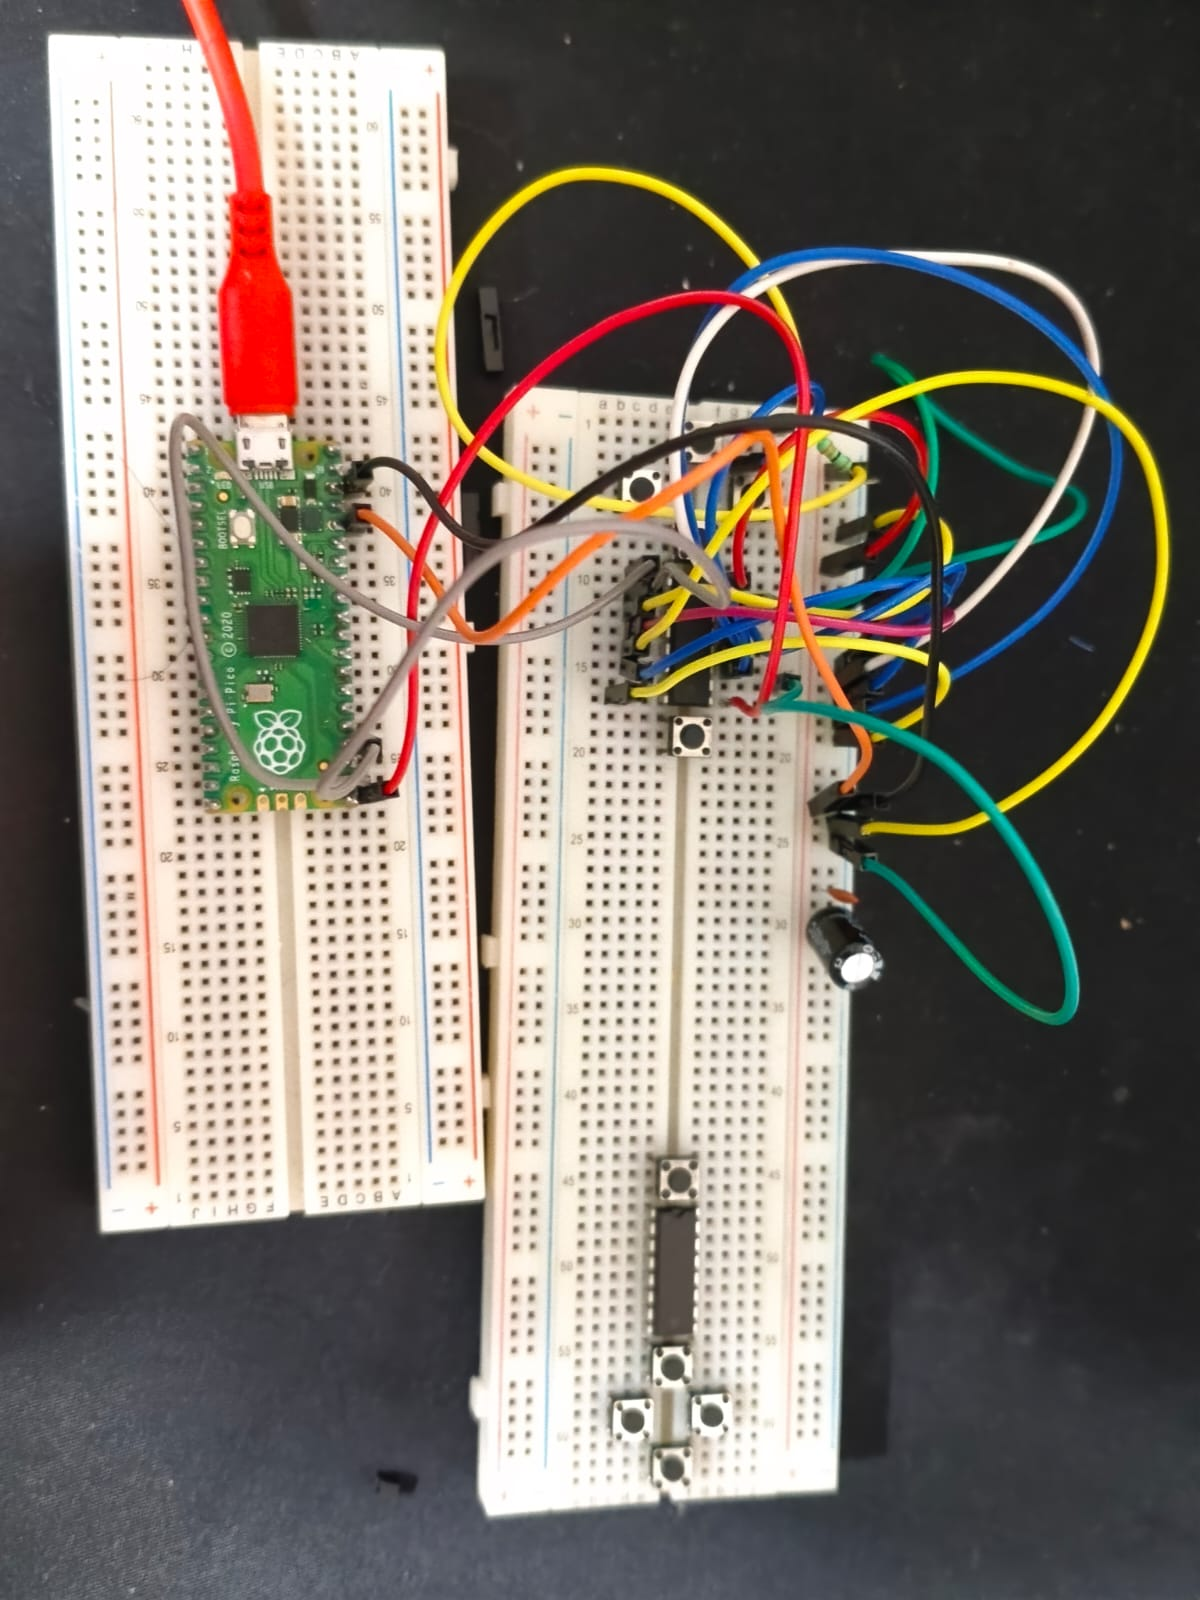
\includegraphics[width=0.62\columnwidth]{img/cableado_foto.png}
	\caption{Prototipo en protoboard.}
	\label{fig:foto}
\end{figure}

\section{Configuración}

\textbf{Máquina PIO.} El programa carga el registro con LD y luego saca los bits con CLK. La PIO corre a $5\text{ MHz}$, así que cada ciclo dura $200\text{ ns}$. Cada bit toma 5 ciclos, lo que da CLK de $1\text{ MHz}$. Una captura de $N$ bits toma $11 + 5N$ ciclos:
\begin{equation*}
	t_8 = 51 \times 200\text{ ns} = 10.2\text{ }\mu\text{s}, \quad
	t_{16} = 91 \times 200\text{ ns} = 18.2\text{ }\mu\text{s}
\end{equation*}

\textbf{Temporizador.} Una alarma de hardware dispara cada $5{,}000\text{ }\mu\text{s}$ con tiempo absoluto, así que un disparo tarde no recorre a los siguientes. Cada captura ocupa solo $10.2 / 5{,}000 = 0.2\%$ del periodo.

\textbf{Antirrebote.} Un cambio se acepta si dos muestras seguidas coinciden, y luego ese botón se bloquea $20\text{ ms}$. El peor retardo es $5 + 5 = 10\text{ ms}$; con $1\text{ ms}$ de USB quedan $11\text{ ms}$, debajo del límite de $15\text{ ms}$.

\textbf{Q7 suelto.} Q7 alterna entre pull-up y pull-down internos en cada captura. Un chip conectado le gana a esa resistencia débil. Si el cable se suelta, la lectura copia la resistencia durante 8 muestras ($40\text{ ms}$), y el módulo reporta la falla y deja de reportar botones.

\textbf{Compilación.} Pico SDK 2.3.1 con \texttt{arm-none-eabi-gcc} 13.2. El binario ocupa $41{,}672\text{ B}$ de Flash y $5{,}624\text{ B}$ estáticos de RAM. Los pasos están en el README.

\section{Pruebas}

La Tabla \ref{tab:pruebas} separa lo que probamos sin la placa de lo que se mide en el hardware. En emulador corrimos el binario real en rp2040js, con un 74HC165 simulado y midiendo LD y CLK desde afuera del firmware. Ese emulador solo simula un núcleo, así que esa compilación usa Core 0 para todo. Por eso los números son una referencia y la columna Hardware es la que confirma el módulo.


\begin{figure}[H]
	\centering
	\imgph{salida de verificar\_modulo.sh con la Pico real}{3.2cm}
	\caption{Verificación en el hardware.}
	\label{fig:hw}
\end{figure}

\section{Decisiones de la bitácora en el código}

Las decisiones están marcadas con \texttt{DECISION BITACORA} en \texttt{firmware/}:
\begin{itemize}
	\item \textbf{Clase 7:} bare-metal, sin SO entre el temporizador y la lectura (\texttt{main.c}).
	\item \textbf{Clase 8:} la interrupción de $5\text{ ms}$ le quita el procesador a lo que esté corriendo (\texttt{adquisicion.c}).
	\item \textbf{Clase 10:} todo es estático, sin heap (\texttt{adquisicion.c}).
	\item \textbf{Clase 12:} la temporización fina la hace un periférico, la PIO (\texttt{adquisicion.c}).
\end{itemize}

Cambiaron tres decisiones del módulo: SPI por PIO, porque el SPI no genera el pulso LD; los papeles de los núcleos, porque el SDK exige el USB serial en Core 0; y mutex por spin lock (Clase 9), porque una interrupción no debe dormirse. El registro completo con motivos está en la bitácora.

\section{Declaración de uso de IA}

En este avance usamos Claude (Anthropic) como apoyo para reorganizar el firmware a partir del código del equipo, escribir los scripts y las pruebas, preparar el emulador y redactar borradores de este reporte y de la bitácora. En el Avance 1 usamos Gemini (Google). Los valores de la columna Hardware los mide el equipo sobre el prototipo.

\vspace{0.2cm}
\noindent\textbf{Repositorio:} \\
\url{https://github.com/SistemasEmbebidos-Grupo6/ProyectoFinal-ArcadeRetro}

\end{document}
